\chapter{Construction of a miniature epi-fluorescence microscope}

\section{Introduction}\todo{edit microscope intro}


    One of the major technological limitation in neuroscience research is recording neural activity in model animals. Traditional techniques such multi-unit recordings give excellent temporal resolution, however the spatial resolution --- as measured by the number of cells simutaneously recorded --- is limited. Moreover, it is very hard to distinguish cell subpopulations within the same region from the recording. Neural activity can also be inferred by post-hoc staining of neural activity markers, such as cfos or arc. This method give excellent spatial resolution, however the temporal resolution is very poor, where the time window of neural activity lasts from minutes to hours.

    Live calcium imaging gives the best of both method. By labelling the cell of interest with a calcium indicator, neural activity can be inferred in milli-second resolution. Hundreds of cells can be simultaneously recorded, and specific subpopulations can be distinguished by fluorescence in different colour channels. However, traditional live calcium imaging requires the animals' head firmly fixed under a microscope stage. This requirement is incompatible with most well established behaviour assays, and at the same time introduce significant stress to the animal, potentially confounding the behavioural result. Moreover, due to light scattering in the opaque brain tissue, most of the studies have focused only on cortical areas, while techniques to image deep brain tissue on a standard two-photon microscope is still under development and not widely adopted \citep{barretto12}.

    \textit{In vivo} calcium imaging in behaving animals is first demonstrated by Mark Schnitzer's group in Stanford \citep{ghosh11}. The authors constructed a miniature epifluorescence microscope which is chronically implanted in the brain to image the fluorescence from region of interest. In a follow-up paper \citep{ziv13}, the authors demonstrated that the miniature microscope can image GCaMP3 calcium signals from hippocampal \gls{ca1} place cells for more than a month. However, there has been several limitations of their design: first their design incorporates an objective lens of \SI{1}{\mm}  in diameter, which is impractical to reach deep brain tissue; second, their mini-microscope was only able to identify GCaMP signals, and therefore unable to distinguish different cells types within the population \citep{ghosh11,ziv13}. 

    In the current project, we aim to tackle the above mentioned limitations by building a head-mount miniature microscope which is able to image calcium signals in deep brain structures, while also able to image a separate fluorescence colour channel, allowing to distinguish difference cell type. The mini-microscope, once developed, will be used for imaging \gls{la} neurons to investigate mechanisms of fear memory encoding.


\section{Material and Methods}

\subsection{Design of the mini-microscope}

The mini-microscope has the same design as an general single-photon epiflourescence microscope except for the size constraints. Excitation light is emitted from a \gls{led} light source, filtered, reflected by a dichroic mirror and evenly illuminate the sample. The flourescent light from the sample is collected by the objective, passes through the dichroic mirror, filtered and focused on the camera. The fit the size constraints, we chose the use a high-intensity \gls{led} as the light source, a \gls{grin} lens as an objective, and a miniatured \gls{cmos} camera to capture the image.\todo{maybe a illustration}

The optical design of the microscope is aided with Zemax software (Zemax Development Corporation) to optimize the lens and filter configuration. The casing of the microscope is modelled using OpenSCAD software. 

\subsubsection{Lens configuration}

The lenses configuration consists a \gls{grin} objective lens and a ocular cube lens forming a 4F system, where the distance between the thin-lens equivelant of the two lenses equals to the sum of the focal length. Potential lenses for emission light path are selected from modelling and calculation to give a working distance of \SI{100}{\um} in water, a magnification of 6x and a back focal length of \SI{6}{\cm}. During prototyping, the lenses are purchased and installed into custom-made mounts on a two-arm stereotaxic frame. The distance of the lenses are then optimized against a fibre bundle light source close to the \gls{grin} lens. A drum lens is used to collect light from the \gls{led}. The drum lens is tested in a similar manner and selected to give diverging light after \gls{grin} lens. We has chose to use an achromatic doublet (F=\SI{15}{\mm}, Edmund Optics). We used a \SI{1.8}{\mm} diameter 0.25-pitch \gls{grin} lens (64--537, Edmund Optics) as objective for hippocampus imaging. To minimize brain damage for deep brain imaging, the objective lens was a home-assembled doublet of a \SI{0.5}{\mm} diameter, 1-pitch \gls{grin} relay lens (\todo{GoFoton lens info}) and a \SI{2}{\mm} diameter 0.25-pitch \gls{grin} lens (\todo{GoFoton lens info}). The details of doublet assembly is described in \label{objective assmebly}.

\subsubsection{Filter selection}
The filters are selected to cover the excitation and emission spectrum of the genetic encoded calcium sensor GCaMP6s \citep{chen13}, and further screen for high bandwidth and low overlap. The fit the size constraints, the excitation and emission filters had dimensions of \SI{5x5x1}{\mm}, and the dichroic mirror \SI{7.1x5x1}{\mm}. We have chose to use a \gls{fitc} filter set for gCaMP6 imaging (\todo{chroma filter info}). For dual colour imaging, we took advantage of significant long tail of the red retrobeads spectrum, and use the same blue light to excite the red flourephore. In these experiments, a \acrshort{tritc}\slash\acrshort{fitc} filter set was used (\todo{chroma filter info}).

\subsubsection{Electronics}
The image sensor are selected to have an packaged size of less than \SI{1.5 x 1.5}{\cm}. We used a commercially available analogue camera module (HD1313BW, Ruishibao) that gives satisfactory sensitivity and dynamic range. The camera board is connected to a \SI{5}{\V} power regulator. After the power regulator, the wires were connected through a slip ring (\todo{slipring info}) was the used to avoid tanglement of the wires during animal behaviour. After the slip ring, the wires are connected to a \SI{12}{\V} \gls{dc} power source and a \gls{usb} analogue video capture card (\todo{Video capture info}). The video capture card is controlled by custom software for synchronized video capture (See code in \todo{reference code}).

A monochrome, high-intensity blue \gls{led} (\todo{led info}, Lumiled) was used as the light source. The \gls{led} wires joins the video camera wires through the slip ring, and then connected to a variable \gls{dc} power source (\todo{DC power source info}). During recording, the \gls{led} was driven at a current between \SI{20}{\mA} and \SI{100}{\mA}.

\subsubsection{Casing and assembly}
The casing model is produced by 3D printing using PolyJet technology with VeroBlackPlus material (Stratasys). This gives a rigid, opaque and black casing with highest resolution for details. The microscope body is screwed onto the camera holder via M8 thread to allow easy change of the focus plane. A side M2$\times$\SI{2}{\mm} nylon screw (\todo{info side screw}) is used to lock the camera holder on the microscope body.

A metal nut \todo{microscope body nut spec} was glued to the bottom of the microscopy body concentric to the light path opening using a fast-curing epoxy glue (\todo{epoxy info?}). The nut allows to easily and firmly lock the microscope onto the baseplate.

Unlike the microscope body, the base plate was 3d printed using \gls{fdm} with \gls{pla} material. A threaded tube (\todo{baseplate thread tube info}) was heated with a soldering iron and inserted into the center of the base plate, and further fixed with epoxy glue. The objective lens was inserted into the center of the threaded tube, and fixed with crazy glue on the bottom. For objective that are thinner than the inner diameter of the threaded tube, an additional stainless steel tube was inserted inbetween to aid alignment of the lens.

\subsubsection{Objective for deep brain imaging} \label{objective assembly}

For deep brain imaging, a \SI{0.5}{\mm} diameter, 1.0-pitch relay lens was glued to a \SI{2}{\mm} diameter, 0.25-pitch \gls{grin} lens. The setup is modified from \citep{kim12} to ensure concentricity and alignment. In the setup, a V-groove clamp (\todo{clamp details}, ThorLab) is used to hold the large \gls{grin} lens in place virtically, and the thin relay lens was mounted on another V-groove clamp attached to a 3-axis manipulator (\todo{manipulator details}, ThorLabs). The two V-groove clamps were leveled using a bull's eye spirit level. An analogue lens and camera chip was mounted under the large \gls{grin} lens, and displayed the image of the large \gls{grin} lens on a monitor. A disecting microscope was mounted horizontally for monitoring the vertical position of the two lenses. \todo{insert figure for the setup}

During assembly, both lenses were mounted in the V-groove clamps respectively. A small drop of \gls{uv} curing optical adhesive (NOA61, Norland) was added to the bottom surface of the relay lens using a 27-gauge needle. The relay lens was then lower to just above the large \gls{grin} lens when an image of the relay lens is visible on the monitor. The relay lens was then moved to the center of the large \gls{grin} lens according to the monitor display. Observed through the dissecting microscope, the relay lens was then lowered to touch the upper surface of the large \gls{grin} lens. A \SI{375}{\nm} spot \gls{uv} light source (\todo{uv light source info}) was used to cure the optical glue. The curing time is calculated to give at least \SI{3}{\J\per\mm\squared} of \gls{uv} light on the optical adhesive. 


\subsection{Implantation of the mini-microscope}

Two weeks after gCaMP6 infusion to the target area, animals are anesthesized and head-fixed on a stereotaxic frame as described in \todo{ref general methods}. Three screws were placed around the viral injection site for anchoring the microscope. 

For implantation targetting \gls{ca1}, a circular craniology of \SI{2}{\mm} was performed above the viral injection site. The dura was pierced and lifted with a fine tweezer to expose the brain. The brain is then constantly irrigated with artificial cerebral-spinal cord fluid to remove the blood. A 27-gauge aspiration needle was used to remove cortex and expose \gls{ca1}. For implantation targetting amygdala after anchoring the screws, a 27-gauge needle was lowered to the target coordinate, left for \SI{5}{\min}, and slowly retracted.

The mini-microscope is then fixed on the stereotaxic frame and gradually lowered to the target coordinates (\gls{ca1}: \gls{la}: \todo{coordinate for ca1 and amygdala}). Opaque black dental acrylic was used to secure the microscope baseplate to the skull. Once the dental acrylic cured, the microscope body was detached from the baseplate and replaced with a cap. Animals were given \SI{5}{\mg\per\kg} ketoprofen for analgesia.

\subsection{In vivo mini-microscope testing}
After lens implantation, the animals were kept in the home cage for at least two weeks before the first image session. This time allows the optical window to clear up. The animals were scruffed, the cap was removed and replaced with the microscope body. A typical imaging session lasts for \SI{5}{\minute}. After the imaging session the microscope body was removed, and the animal was recapped.

\subsection{Image analysis}
Individual cell calcium signals were extracted from the movie as previously described \citep{mukamel09}. Briefly, we first estimate the number of cells in the movie, and reduced the number of temporal dimension to roughly number of cells using principle component analysis. The resulting principle components were then subjected to independent component analysis, where the spatial filter for individual cells were extracted from the components, and the calcium signal of the corresponding cell was extracted from the mixing matrix. The time-course calcium signal was then aligned with behaviour recordings to identify neural activity patterns.


\section{Results}\todo{edit microscope result}

With the design from \citet{ghosh11} as a guide, we started to make our own epifluorescence mini-microscope. Currently we have constructed working prototypes weighing less than \SI{3}{\g}, and can be bounded in a \SI{25 x 16 x 11}{\mm} box. The light source is a high intensity blue \gls{led} (LXML--PB01--0023, Lumileds). The illumination light is collected by a drum lens (45--549, Edmund Optics) and then filtered by a blue bandpass filter (ET470/40x, Chroma). The filtered illumination is then reflected by a dichroic mirror (T495lpxr, Chroma) on to the sample. Fluorescence is collected by a \SI{1.8}{\mm} \gls{grin} lens (64--537, Edmund Optics), filtered with a green bandpass filter (ET525/50m, Chroma), then focused by an achromatic lens (49--277, Edmund Optics) onto a 600 tv-line analogue CMOS camera sensor (ASX340, Aptina). The analogue signal is then converted by a consumer video capture device (MyGica) at resolution of \num{720 x 576} and a frame rate of 25 frames per second.

An image of the mini-microscope is shown in Figure~\ref{f.scope}. The resolution of the microscope is better than \SI{2}{\um}, as shown in Figure~\ref{f.usaf} when it is tested against USAF resolution target (Lines in group 7 element 6 have width of \SI{2.07}{\um} and are clearly visible). We have tested the prototype on a perfused brain with \gls{gfp} signals. And as shown in \ref{f.scope-gfp}, the \gls{gfp} cells are clearly identified, with some of the neural processes visible.

To test \textit{in vivo} imaging capability of the microscope, we first implanted the microscope above the cortex, and injected \SI{150}{\ul} of fluorescein-dextran (molecular weight \SI{120}{\kilo\dalton}). The fluorescein-dextran will fill the blood vessels and have similar excitation and emission wavelength to GCaMP. As expected, after fluorescein-dextran injection, the blood vessels are clearly visible when the microscope is implanted (Figure~\ref{f.bloodvessel}).

We have first tested GCaMP6s fluorescence \textit{in vitro}. HEK--293 cells were transfected with pGP--CMV--gCAMP6s (Addgene), and imaged the next day. During imaging session, we challenged the cell with \SI{10}{\nmol} ATP, which is known to up-regulate intra-cellular \ce{Ca^2+} level \citep[\textit{e.g.}][]{lee04}. The result is shown in Figure~\ref{f.gcampinvitro}. The GCaMP6s gives minimal background but bright fluorescence when the intracellular \ce{Ca^2+} is induced.

To test GCaMP6s expression \textit{in vivo}, we infused AAV--syn--GCaMP6s--WPRE into CA1 hippocampus of animals. After AAV expression plateaued, we aspirated cortical tissue above the viral infusion site and implanted the microscope baseplate. After two weeks when the animals recovered and the cranial window was cleared, the microscope was re-attached to the implanted baseplate. The animal were placed in a novel environment to explore for \SI{5}{\minute}, during which GCaMP6 fluorescence were recorded. The maximum projection of the GCaMP6 fluorescence in a 5-minute session is shown in Figure~\ref{f.ca1bw}. More than 200 cells are clearly identifiable.

We used a previously established method to extract \ce{Ca^2+} signals from the movie \citep{mukamel09}. Briefly, we used principle component analysis to reduce the temporal dimension, and then independent component analysis to extract the spatial location of cells and their corresponding \ce{Ca^2+} signals. Figure~\ref{f.analysis} shows a sample independent component that represents a cell and it's activity. The extracted cells are random coloured in Figure~\ref{f.ca1rainbow}.   

The timecourse of the identified cells were mapped back to the behaviour of the animal. Figure~\ref{f.traceplot} shows \ce{Ca^2+} activity of potential place cells as they respond to specific location in the environment the animal is in.

This design of the miniature microscope incorporates an objective lens of \SI{1.8}{\mm} in diameter. This lens is both too thick and too short to reach deep brain structures such as amygdala. We have modified the design and attached a \SI{4.8}{\mm} long \SI{0.5}{\mm} diameter relay \gls{grin} lens (ILW-050-P050, GoFoton) to the objective lens. Attaching the relay lens does not significantly alter the imaging ability of the microscope, however allows the lens to reach deep brain regions without extensive damage. With this configuration, we are able to visualize activity form more than 40 cells in lateral amygdala and track them over time (Figure~\ref{f.amygdala}).


To enable us to identify different cell types in a population, we decided to add a second colour channel in the microscope. We have switched the filter set to a FITC/TRITC dual band set (Chroma 59004), and also from grayscale camera to an RGB camera chip. Figure~\ref{f.twocolour} shows the two-colour microscope against perfused brain expressing \gls{gfp} and TdTomato. Both fluorophore can be clearly seen. We have also tested the red channel \textit{in vivo}, where we infused red retrobeads (LumaFlour) in \gls{nac} and implanted the mini-microscope in \gls{la}. The retrobeads travels retrogradely, and will label amygdala neurons that have connection to \gls{nac}. These cells can be clearly identified under the mini-microscope in the red channel, with no interference to the green channel (Figure~\ref{f.twocolour.g.invivo},\ref{f.twocolour.r.invivo}). 



\begin{figure}[h]
    \begin{subfigure}[t]{.55\textwidth}
        \centering
        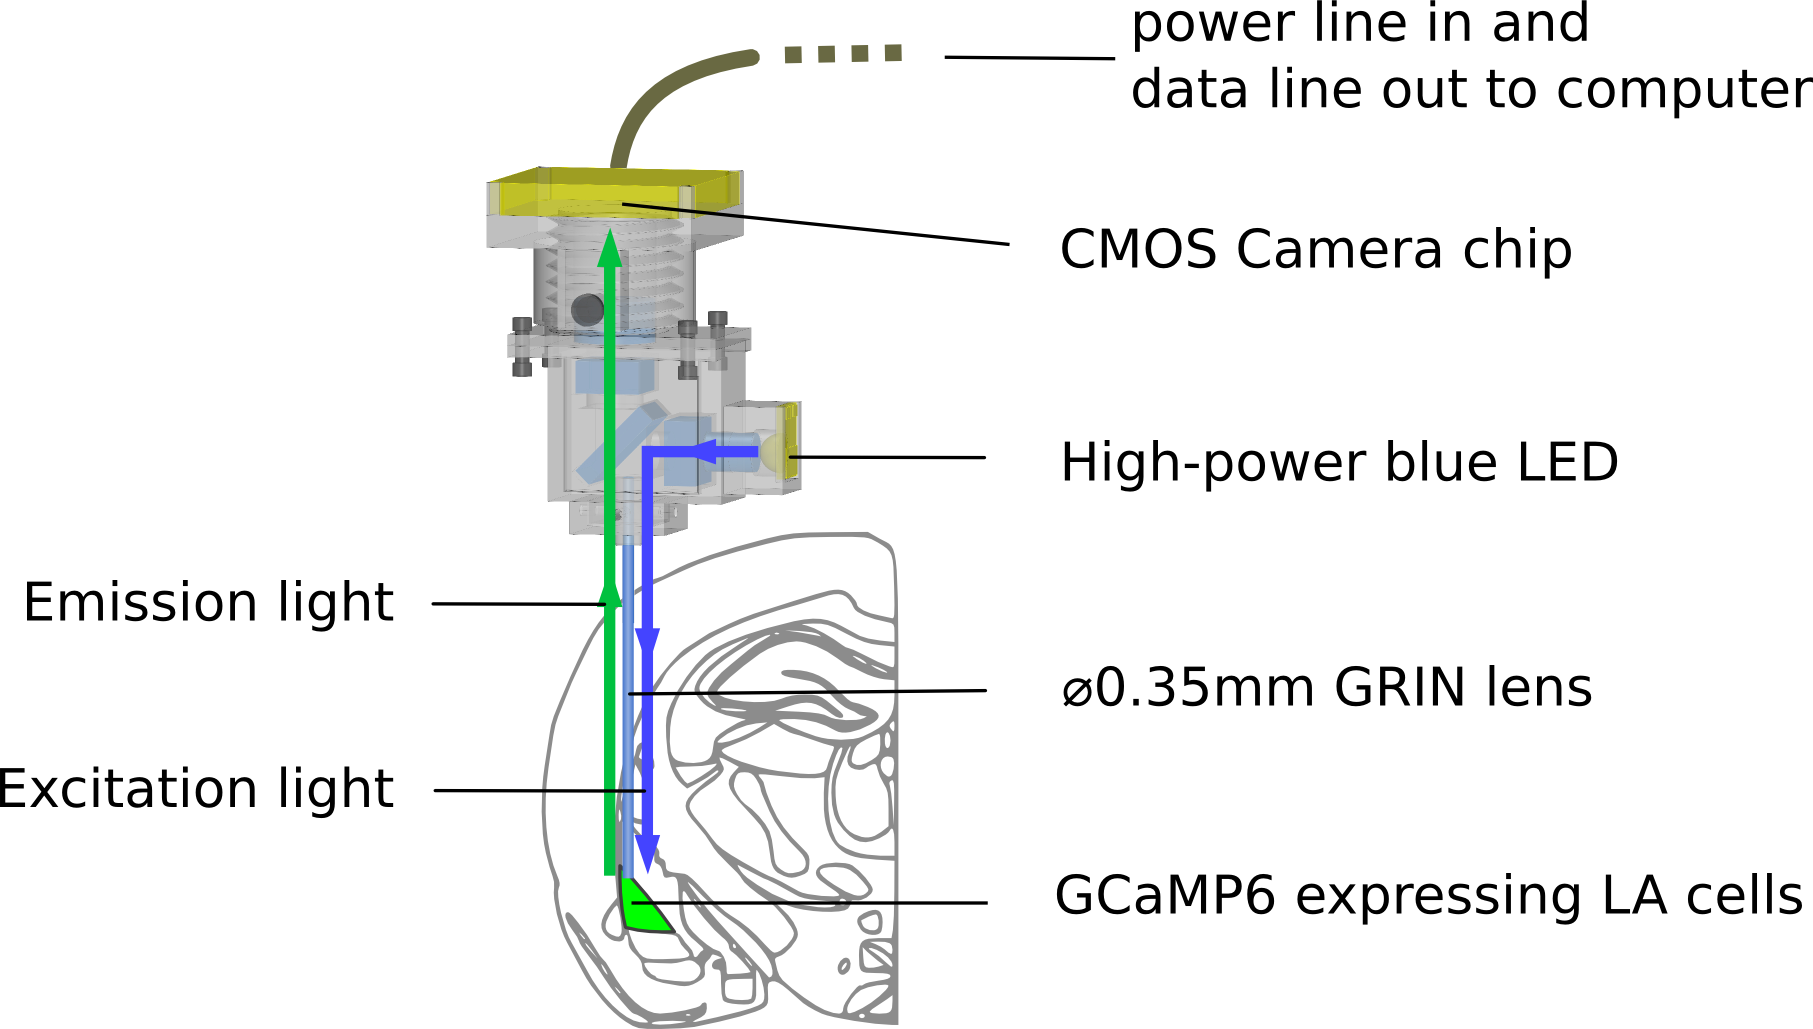
\includegraphics[width=\textwidth]{microscope-schematic.png}
        \caption{\label{f.scope-schema}}
    \end{subfigure}
    \begin{subfigure}[t]{.45\textwidth}
        \centering
        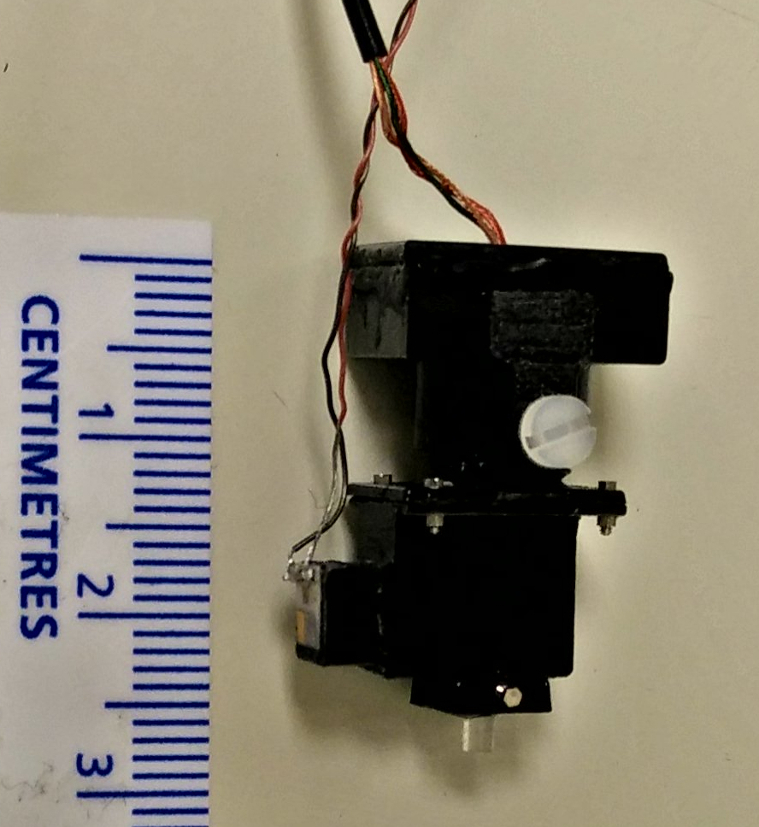
\includegraphics[width=\textwidth]{scope-cropped.jpg}
        \caption{\label{f.scope}}
    \end{subfigure}
    \begin{subfigure}[t]{.5\textwidth}
        \centering
        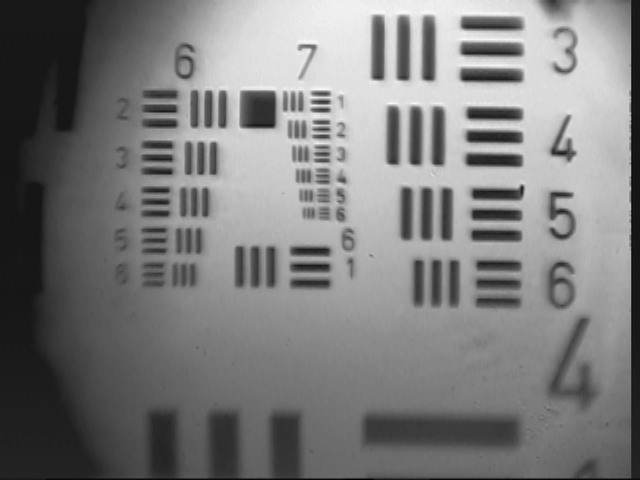
\includegraphics[width=\textwidth]{usaf-target.png}
        \caption{\label{f.usaf}}
    \end{subfigure}
    \begin{subfigure}[t]{.5\textwidth}
        \centering
        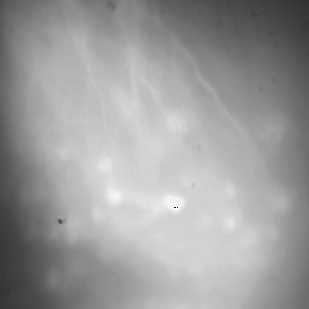
\includegraphics[width=\textwidth]{scope-gfp.png}
        \caption{\label{f.scope-gfp}}
    \end{subfigure}
    \caption{\subref{f.scope-schema} Schematic of the miniature microscope. Excitation light is emitted from a high-intensity blue LED, filtered and reflected to the sample by a dichroic mirror. GCaMP6 emission is collected by the gradient-index (GRIN) lens, filtered and focused onto a CMOS camera chip, where the images are sent to a computer and recorded. 
             \subref{f.scope} Prototype of the mini-microscope.
             \subref{f.usaf} USAF resolution test target under the mini-microscope.}
             \subref{f.scope-gfp} GFP-expressing cells in perfused brain under the miniature microscope.
\end{figure}

\begin{figure}[h]
    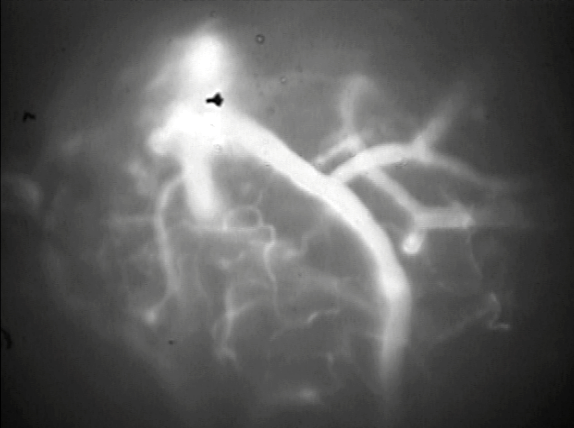
\includegraphics[width=\textwidth]{blood-vessel.png}
    \caption{\textit{In vivo} image of blood vessel. The animal received 10mg/kg fluorescein-dextran in tail vein. The mini-microscope is placed at cortex when the animal is under anaesthesia. \label{f.bloodvessel}}
\end{figure}


\begin{figure}[h]
    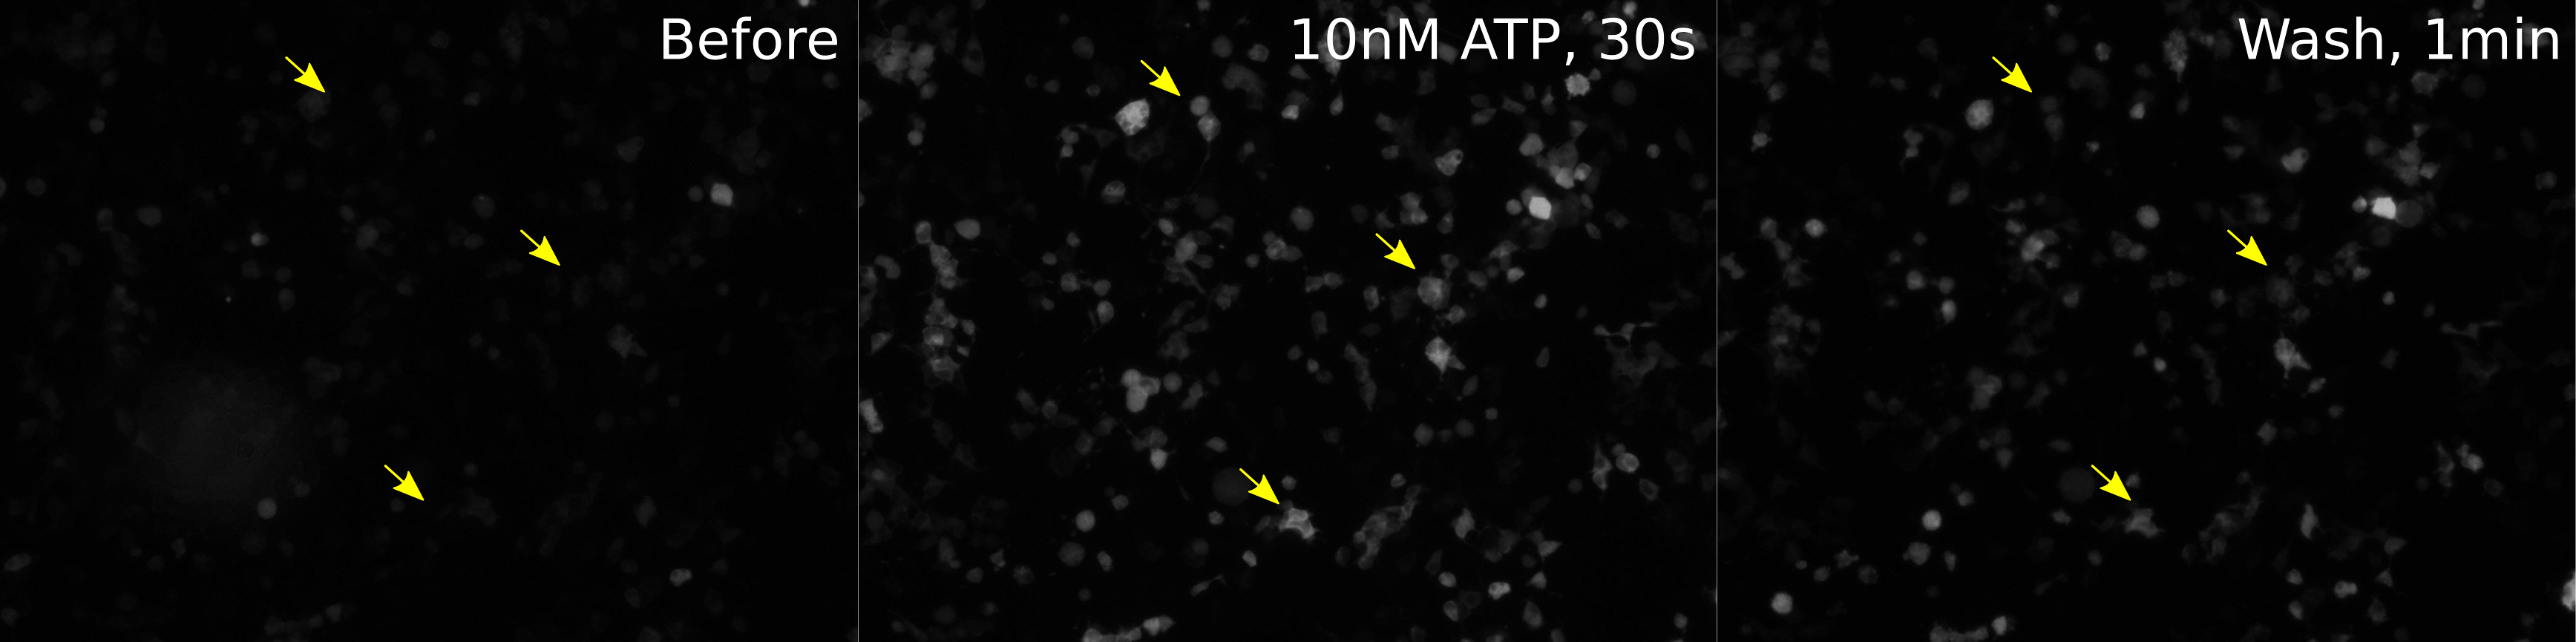
\includegraphics[width=\textwidth]{gcamp-in-vitro.jpg}
    \caption{Expression of GCaMP6s \textit{in vitro}. HEK--293 cells were transfected with pGP--syn--GCaMP6s--WPRE. During imaging session, the cells are challenged with 10nM ATP to induce intracellular \ce{Ca^2+}. Images are taken from an inverted light microscope. GCaMP6s gives minimum background, and shows significant fluorescence when intracellular \ce{Ca^2+} is induced. \label{f.gcampinvitro}}
\end{figure}


\begin{figure}[h]
    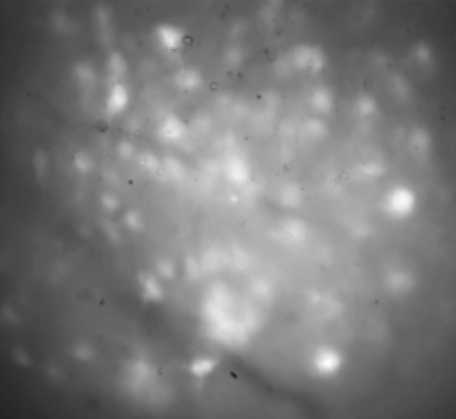
\includegraphics[width=\textwidth]{cells-bw.png}
    \caption{Cells in CA1 captured by the mini-microscope in behaving animal. Two weeks after AAV infusion and microscope implantation, the animal is allowed to freely explore a novel environment. The picture is a maximum projection of all frames captured in a 5-minute session. \label{f.ca1bw}}
\end{figure}

\begin{figure}[h]
    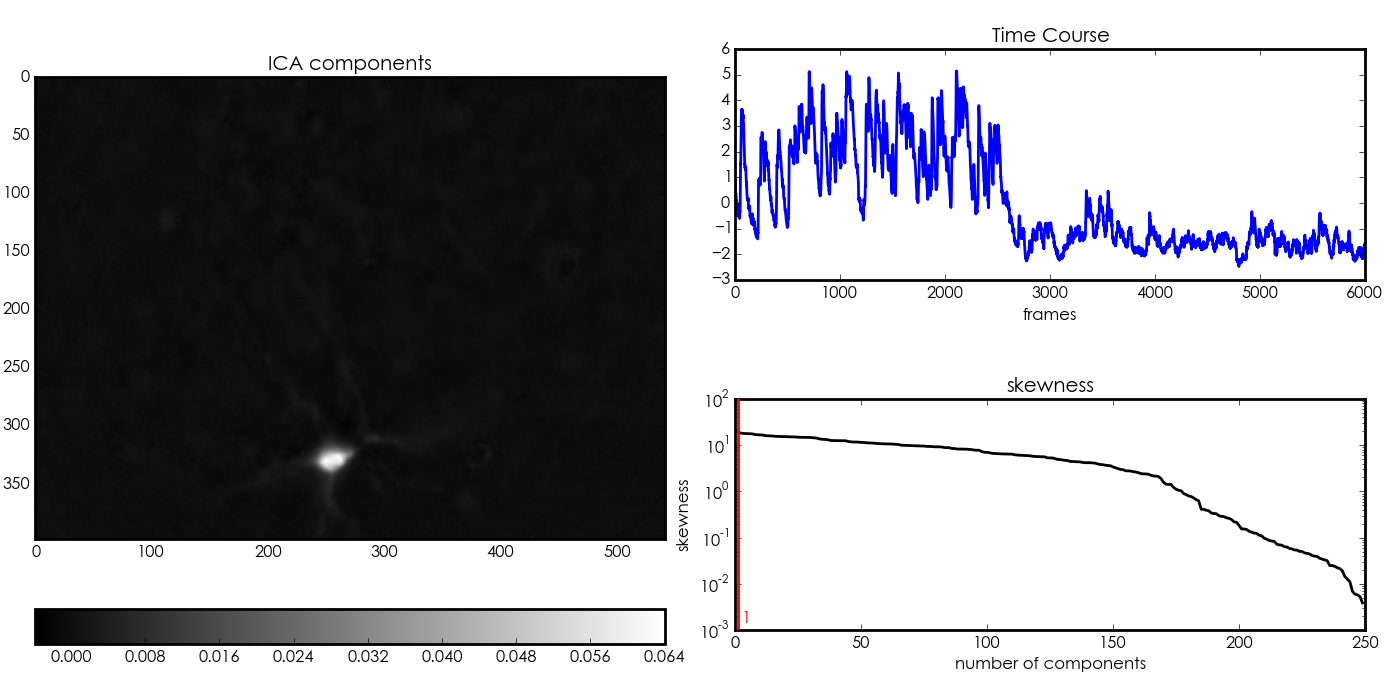
\includegraphics[width=\textwidth]{analysis1.png}
    \caption{Example of an independent component of the movie after analysis, showing both the extracted spatial location of the cell (left) and the un-normalized actvity (top right). \label{f.analysis}}
\end{figure}


\begin{figure}[h]
    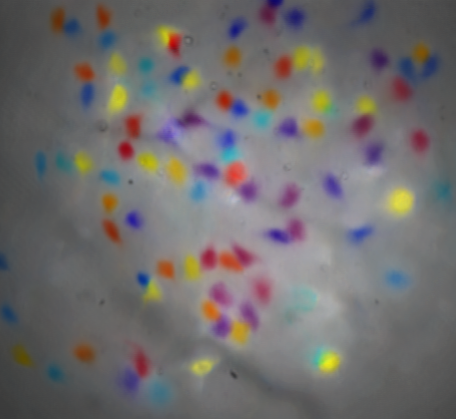
\includegraphics[width=\textwidth]{cells-bw-rainbow-all-final.png}
    \caption{More than 100 cells are identified in a single imaging session. The identified cells are randomly coloured. \label{f.ca1rainbow}}
\end{figure}


\begin{figure}[h]
    \begin{subfigure}[t]{.5\linewidth}
        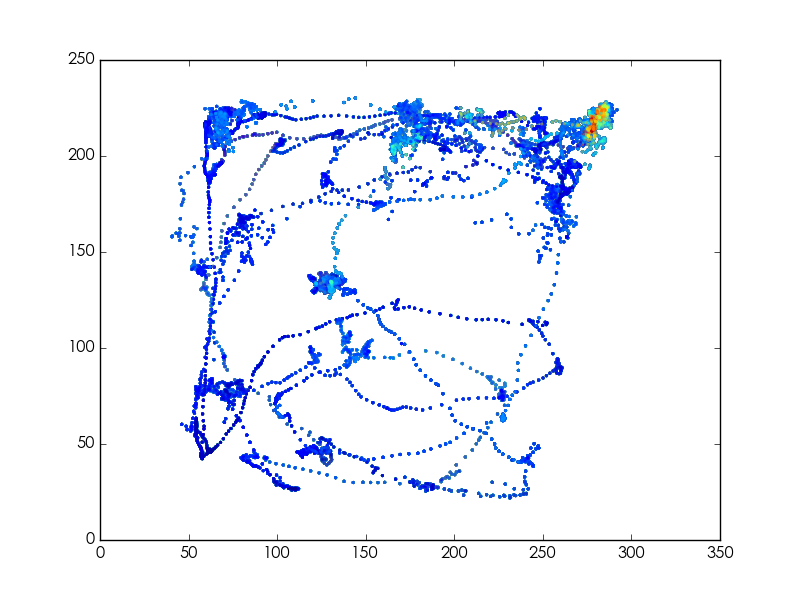
\includegraphics[width=\textwidth]{trace1.png}
    \end{subfigure}
    \begin{subfigure}[t]{.5\linewidth}
        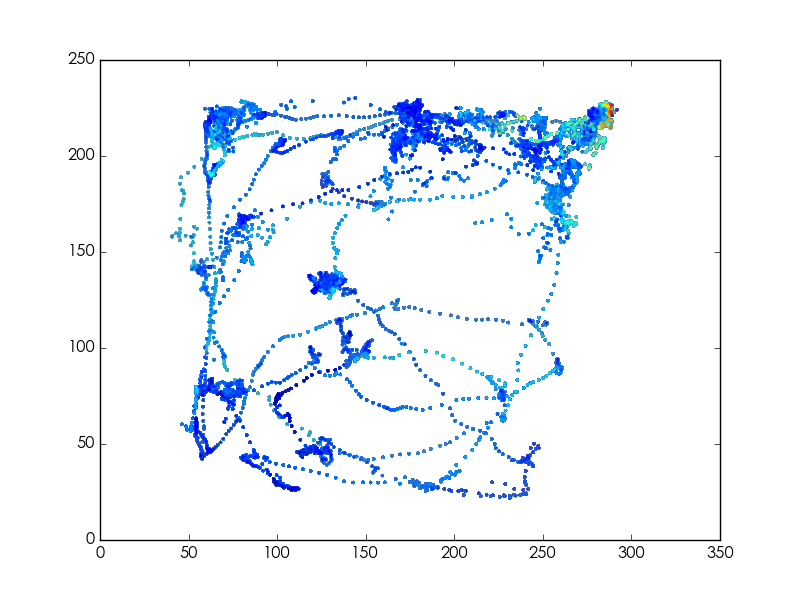
\includegraphics[width=\textwidth]{trace2.png}
    \end{subfigure}
    \begin{subfigure}[t]{.5\linewidth}
        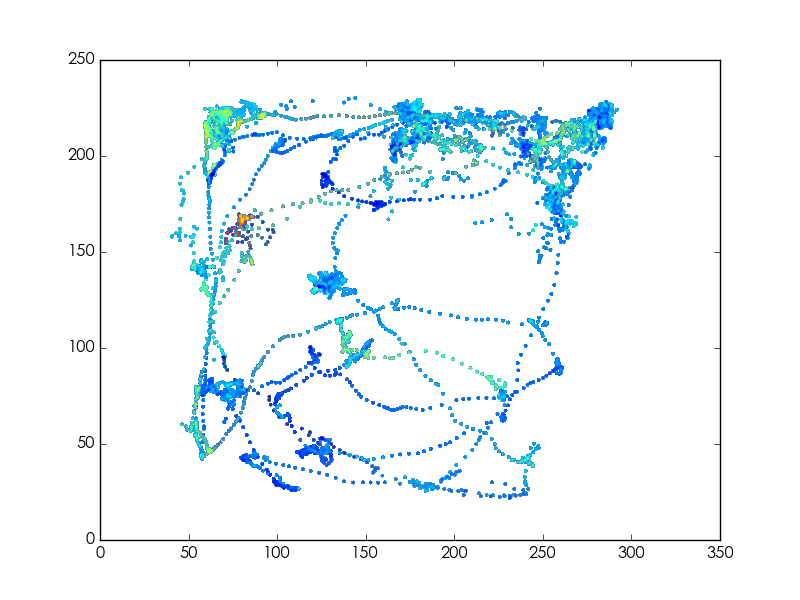
\includegraphics[width=\textwidth]{trace3.png}
    \end{subfigure}
    \begin{subfigure}[t]{.5\linewidth}
        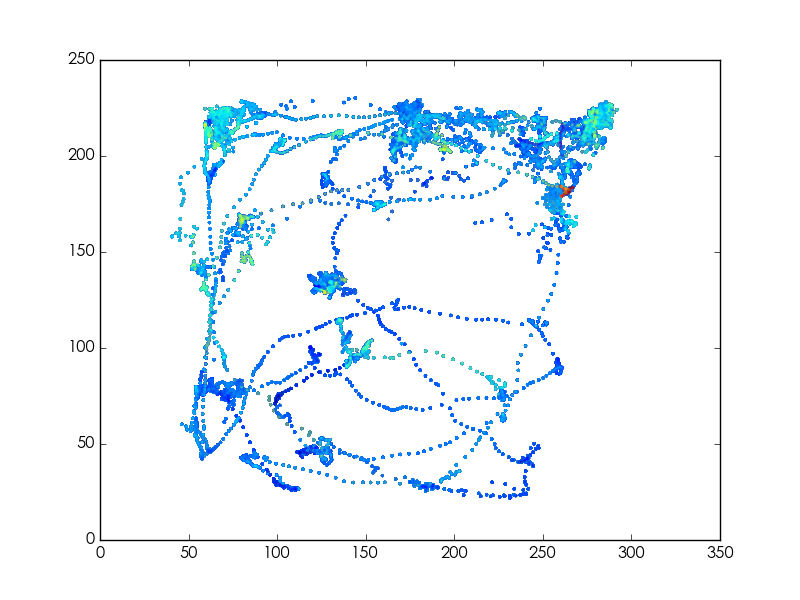
\includegraphics[width=\textwidth]{trace4.png}
    \end{subfigure}
    \caption{Activity of 4 sample cells plotted against location of the animal. The colour represents the \ce{Ca^2+} activity. The cellular activity is specific to the animal's location in the environment. \label{f.traceplot}}
\end{figure}

\begin{figure}[h]
    \centering
    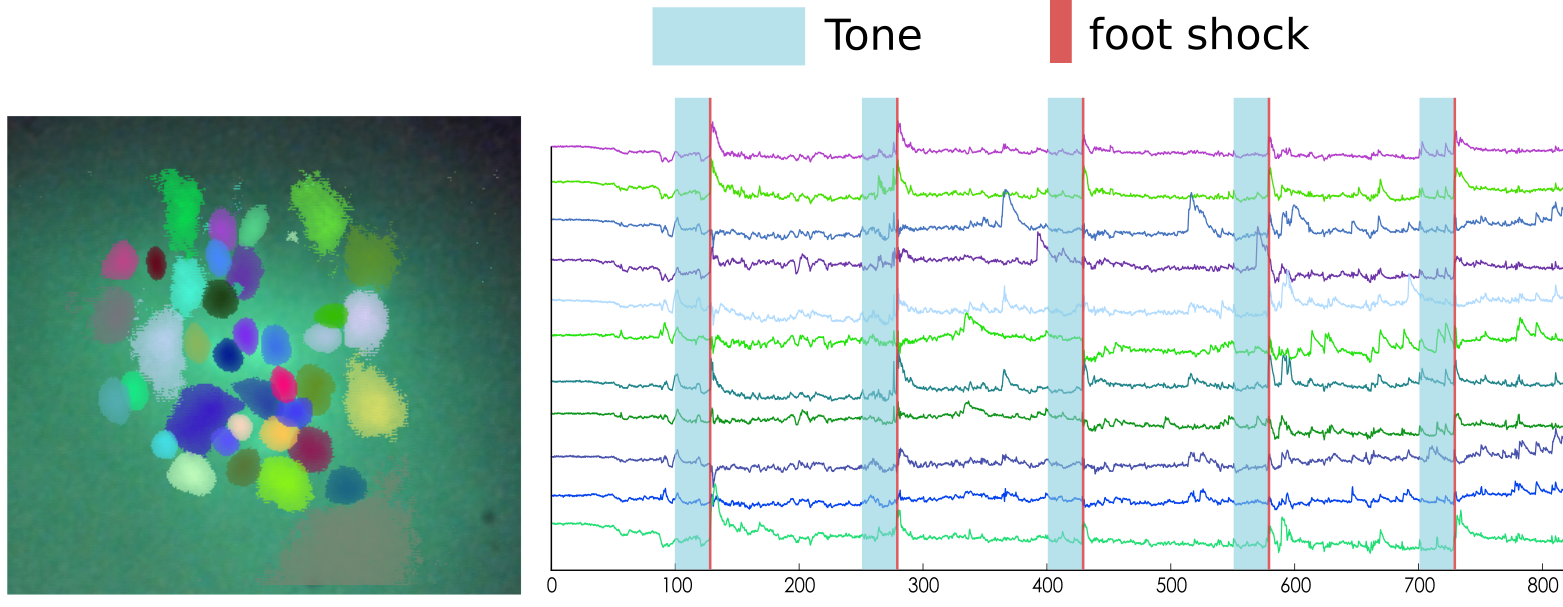
\includegraphics[width=\textwidth]{amygdala.png}
    \caption{Raw calcium signals during fear conditioning. Left: extracted map of neurons, randomly coloured. Right: Sample calcium signals over time.\label{f.amygdala}}

\end{figure}

\begin{figure}[h]
    \begin{subfigure}[t]{.5\linewidth}
        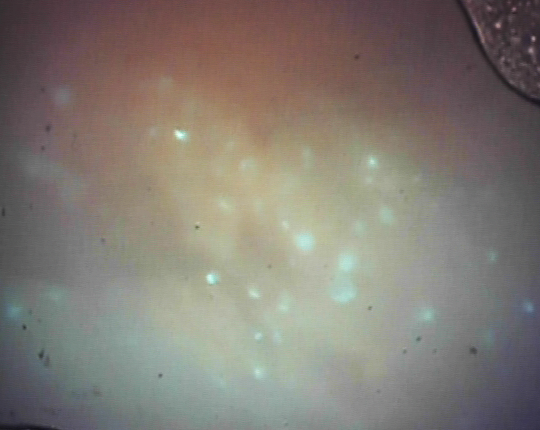
\includegraphics[width=\textwidth]{two-colour-g.png}
        \caption{\label{f.twocolour.g}}
    \end{subfigure}
    \begin{subfigure}[t]{.5\linewidth}
        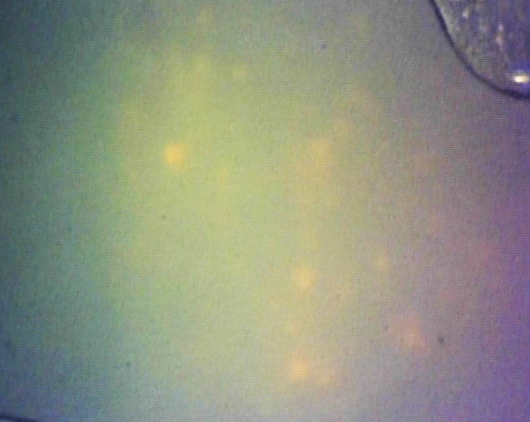
\includegraphics[width=\textwidth]{two-colour-r.png}
        \caption{\label{f.twocolour.r}}
    \end{subfigure}
    \begin{subfigure}[t]{.5\linewidth}
        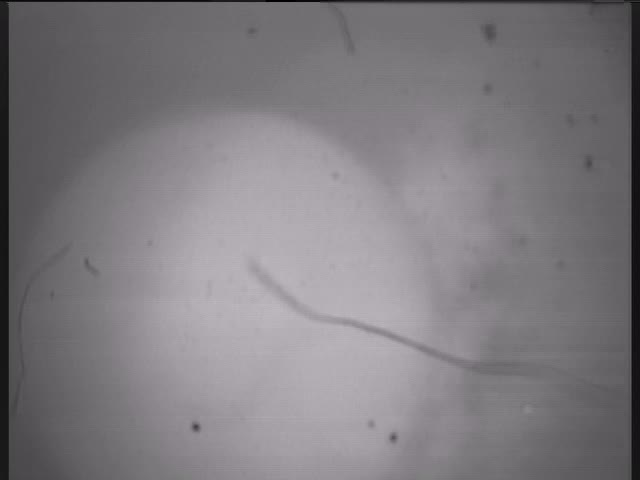
\includegraphics[width=\textwidth]{two-colour-green-in-vivo.png}
        \caption{\label{f.twocolour.g.invivo}}
    \end{subfigure}
    \begin{subfigure}[t]{.5\linewidth}
        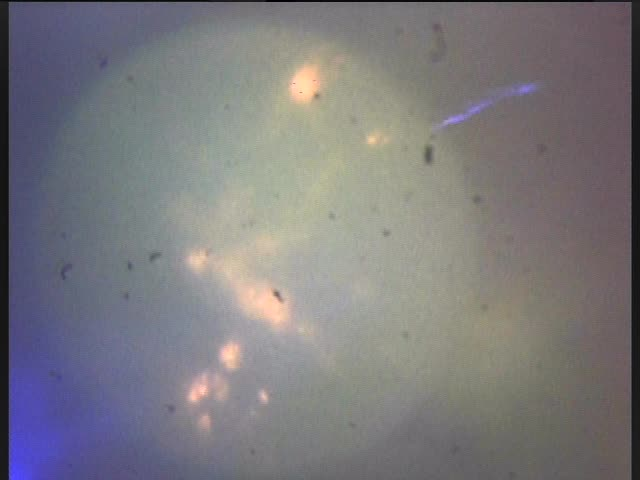
\includegraphics[width=\textwidth]{two-colour-red-in-vivo.png}
        \caption{\label{f.twocolour.r.invivo}}
    \end{subfigure}

    \caption{Images of cells with different fluorescent protein under the two-colour mini-microscope prototype. \subref{f.twocolour.g} HSV-GFP in perfused brain. \subref{f.twocolour.r} HSV-tdTomato in perfused brain. \subref{f.twocolour.g.invivo} Red retrobeads \textit{in vivo} in green channel. \subref{f.twocolour.r.invivo} Red retrobeads \textit{in vivo} in red channel. \label{f.twocolour}}
\end{figure}


\begin{figure}[h]
    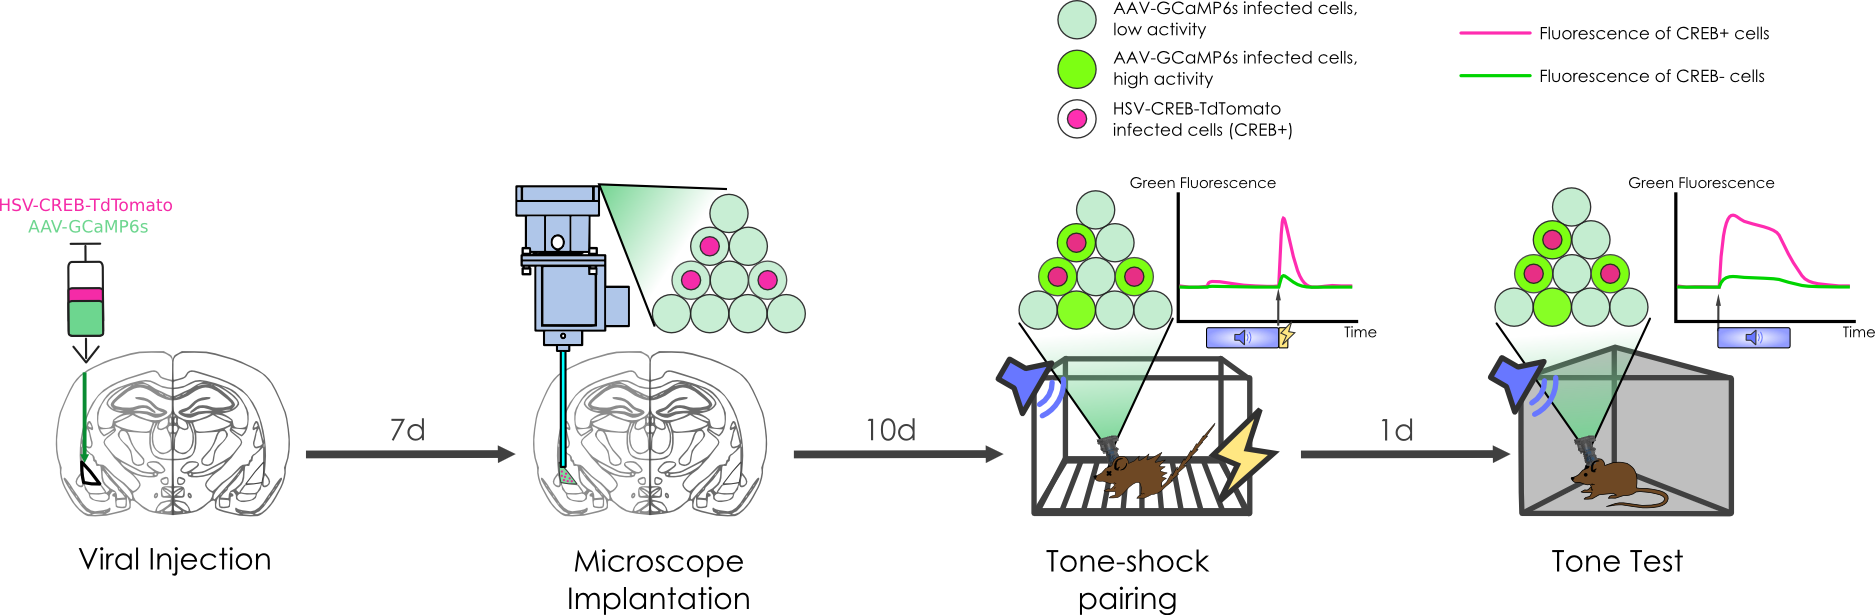
\includegraphics[width=\textwidth]{behaviour-schematic.png}
    \caption{Proposed experiment. A mixture of GCaMP6s-expressing AAV and tdTomato-expressing long-term HSV are infused into LA of the animals. A two-colour microscope is implanted to visualize infected LA neurons. The animal then subject to auditory fear conditioning paradigm, and GCaMP6s signals in either tdTomato\textsuperscript{+} or tdTomato\textsuperscript{-} cells are recorded. We hypothesize that the tdTomato\textsuperscript{+} cells will be more excitable than tdTomato\textsuperscript{-} cells during training and testing. \label{f.behaviour-schema}}
\end{figure}




\section{Discussion}
